\documentclass[12pt, pdflatex]{article}
\usepackage[a4paper, top=3cm, bottom=3cm, right=3cm, left=3cm]{geometry}
\usepackage[french]{babel}
\usepackage[utf8]{inputenc}
\usepackage[T1]{fontenc}
\usepackage[a4paper]{geometry}
\usepackage{amsmath}
\usepackage{graphicx} 
\usepackage{tabularx}
\usepackage{listings}
\usepackage{float}
\usepackage{caption}
\usepackage{parskip}
\usepackage{menukeys}
\usepackage{url}
\usepackage{wrapfig}
\usepackage{hyperref}


\setlength\parindent{24pt}
\newmenumacro{\nixfile}[/]{hyphenatepaths}
\newmenumacro{\nixpath}[/]{hyphenatepathswithfolder}
\newmenumacro{\winpath}[bslash]{hyphenatepathswithfolder}
\newmenumacro{\winfile}[bslash]{hyphenatepaths}


\title{Rapport projet conception logicielle avancée}
\author{VU Nguyen Phuong Vy}

\date{\today}

\begin{document}


\begin{titlepage}
    \centering
    
\includegraphics{sources/logo-unicaen.png}\par\vspace{1cm}
    {\scshape\LARGE Rapport projet conception logicielle avancée \par}
    \vspace{1cm}
    {\scshape\LARGE Ricochet Robots\par}
    \vspace{1cm}
	{\large Nguyen Phuong Vy VU\par}
    \vspace{11cm}
    {\large L2 Informatique - Groupe 2A - Année 2020-2021\par}
	{\large \today \par}

\end{titlepage}

\pagebreak

\tableofcontents

\pagebreak
\section{Introduction}
    \subsection{Ricochet Robots}

    \begin{wrapfigure}{R}{0.45\textwidth}
        \centering
        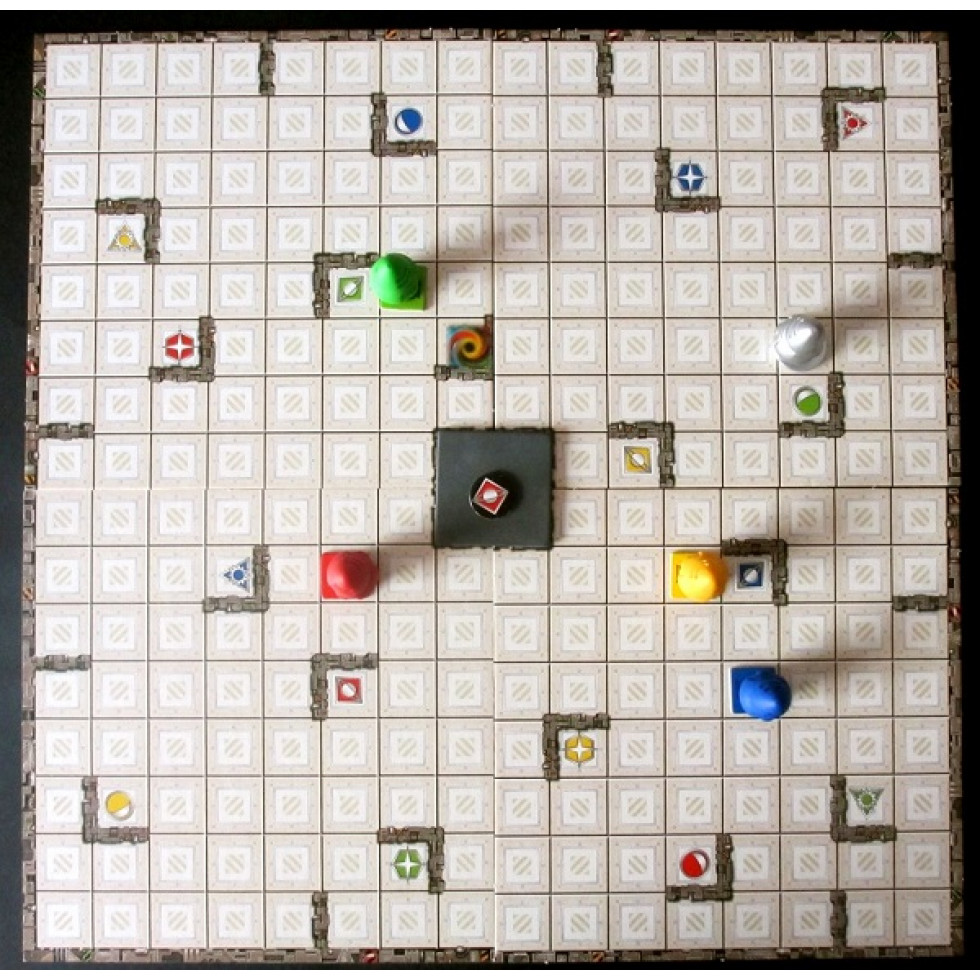
\includegraphics[width=0.4\textwidth, trim=0pt 0pt 0pt 30pt]{sources/rr-orig.jpg}
        \caption{Ricochet Robots}
        \vspace{-20pt}
    \end{wrapfigure}

    En 1999 Hans im Glück / Tilsit ont édité un jeu de société qui a été créé par Alex Randolph et illustré par Franz Vohwinkel. Il est Ricochet Robots. 
    D'après Wikipédia\cite{wiki} le jeu est composé d'un plateau, de tuiles représentant chacune une des cases du plateau, et de pions appelés « robots ». 

    Le jeu se décompose en tours, un tour de déplacement des robots sur le plateau pour en amener un sur l'une des cases du plateau. Les robots se déplacent en ligne et avancent jusqu’à rencontrer un obstacle (un robot ou un mur).

    À chaque tour, l'un des joueurs a remis une tuile cible. Le but est alors de faire en sorte que le robot de la couleur de la tuile sur la case cible dont le symbole est même que le symbole tuile. Si la tuile multicolore est tirée, le but est d'amener n'importe quel robot sur la case multicolore du plateau.
    
    La tuile est remportée par le joueur qui a la solution comptant le moins de mouvement dans délai de temps impartis. Le jeu se termine lorsque tous les jetons auront été tirés. Le gagnant est la personne qui aura récolté le plus jetons.

    Le Ricochet Robots peut aussi bien être joué seul qu’avec un grand nombre de participants.



    \subsection{But du projet}
    Dans ce projet, on a développé un programme qui permet de trouver la meilleure solution pour toute situation du jeu. On a lancé un planning de la conception de ce projet en plusieurs temps :

    \begin{itemize}
        \item Lancer de la conception du projet (diagramme, librairie, méthode)
        \item Développer l'interface du jeu
        \item Développer du moteur du jeu, selon les règles du jeu
        \item Implémenter l'algorithme A* pour chercher le chemin le plus court
        \item Optimiser les méthodes de l'algorithme et vérifier le code pour éviter les bugs
    \end{itemize}

\pagebreak

\section{Organisation du projet}
    \subsection{Hébergement du code}
    On a choisit le forge d'Unicaen pour faciliter la gestion du projet. Il permet de créer et d'administrer des dépôts sous le forge que l'on peut en faire avec terminal. De plus, le forge offre les autres fonctionnalités qui sont une gestion des permissions, une visualisation des différents commits, le suivi de l’activité du projet, etc. 

    \subsection{Tableau des tâches}
    \begin{center}
        \begin{tabular}{|p{5cm}|p{9cm}|}\hline
            \textbf{Classes}& \textbf{Tâches}\\ \hline\hline
            \textbf{Création des modèles}& \\ \hline
            Case&  Contenir un point des coordonnées\\ &Créer des murs et des variables nécessaires     \\ \hline
            Robot&  Distinguer entre la classe Target    \\ \hline
            Target&  Distinguer entre la classe Robot   \\ \hline
            Name& Énumération des symboles différents des targets \\\hline

            \textbf{Création du plateau}& \\\hline
            Board& Construire les éléments \\ &Initialiser les éléments\\ &Déplacer les robots \\ &Rechercher les targets\\ &Réinitialiser le plateau \\ &Exécuter A* \\ \hline
            Direction& Énumération des quatres directions \\\hline

            \textbf{Création de MVC}& \\\hline 
            Draw&  Dessiner l'interface \\ &Déplacer le robot avec clavier \\ &Sélectionner le robot avec souris \\ &Lancer A*      \\ \hline
            
            \textbf{Algorithme A*}& \\\hline
            AStar& Créer une liste des coups validés\\ &Initialiser les valeurs heuristiques sur chaque cases \\ &Implémenter A* \\ &Récupérer la liste des cases du chemin \\\hline

            \textbf{Main}& Lancer le jeu\\\hline
            

        \end{tabular}
    \end{center}



\pagebreak

\section{Architecture du projet}
    \subsection{Directoires du projet}
    La structure du projet est non seulement de diviser le projet en des parties spécifiques, mais encore doit adopter la structure de Gradle. Il est structuré en quatre parties.

    \begin{minipage}{\textwidth}
        \begin{tabbing}
        \hspace{1em}\=\hspace{1em}\=\hspace{1em}\=\hspace{12em}\=\\\kill
        \nixpath{assets } \>\>\>\> \\

        \nixpath{expression/rapport    } \>\>\>\> \\

        \nixpath{gradle/wrapper    } \>\>\>\> \\
        
        \nixpath{src/main/java    } \>\>\>\> \+\\
        \nixpath{board  }   \>\>\>   \+\\
        \nixfile{Board.java}     \>\> \\
        \nixfile{Direction.java}     \>\> \-\\

        \nixpath{draw}   \>\>\>  \+\\
        \nixfile{Draw.java}     \>\>  \-\\

        \nixpath{model}   \>\>\>  \+\\
        \nixfile{Case.java}     \>\> \\
        \nixfile{Name.java}     \>\>  \\
        \nixfile{Robot.java}     \>\>  \\
        \nixfile{Target.java}     \>\>  \-\\

        \nixpath{solve}   \>\>\>  \+\\
        \nixfile{AStar.java}     \>\> \-\\

        \nixfile{Main.java}   \>\>\>  \\

        \end{tabbing}
        \end{minipage}
        \par
        On remarque les packages utilisés:
        \begin{itemize}
            \item board: initialiser le plateau avec les robots, les tuiles et les fonctions du jeu
            \item draw: dessiner le plateau, ajouter l'écouteur de clavier et l'écouteur de souris
            \item model: créer modèle du jeu
            \item solve: implémenter l'algorithme A*
        \end{itemize}

    
    \subsection{Diagramme des classes}
    \begin{figure}[H]
        \centering
        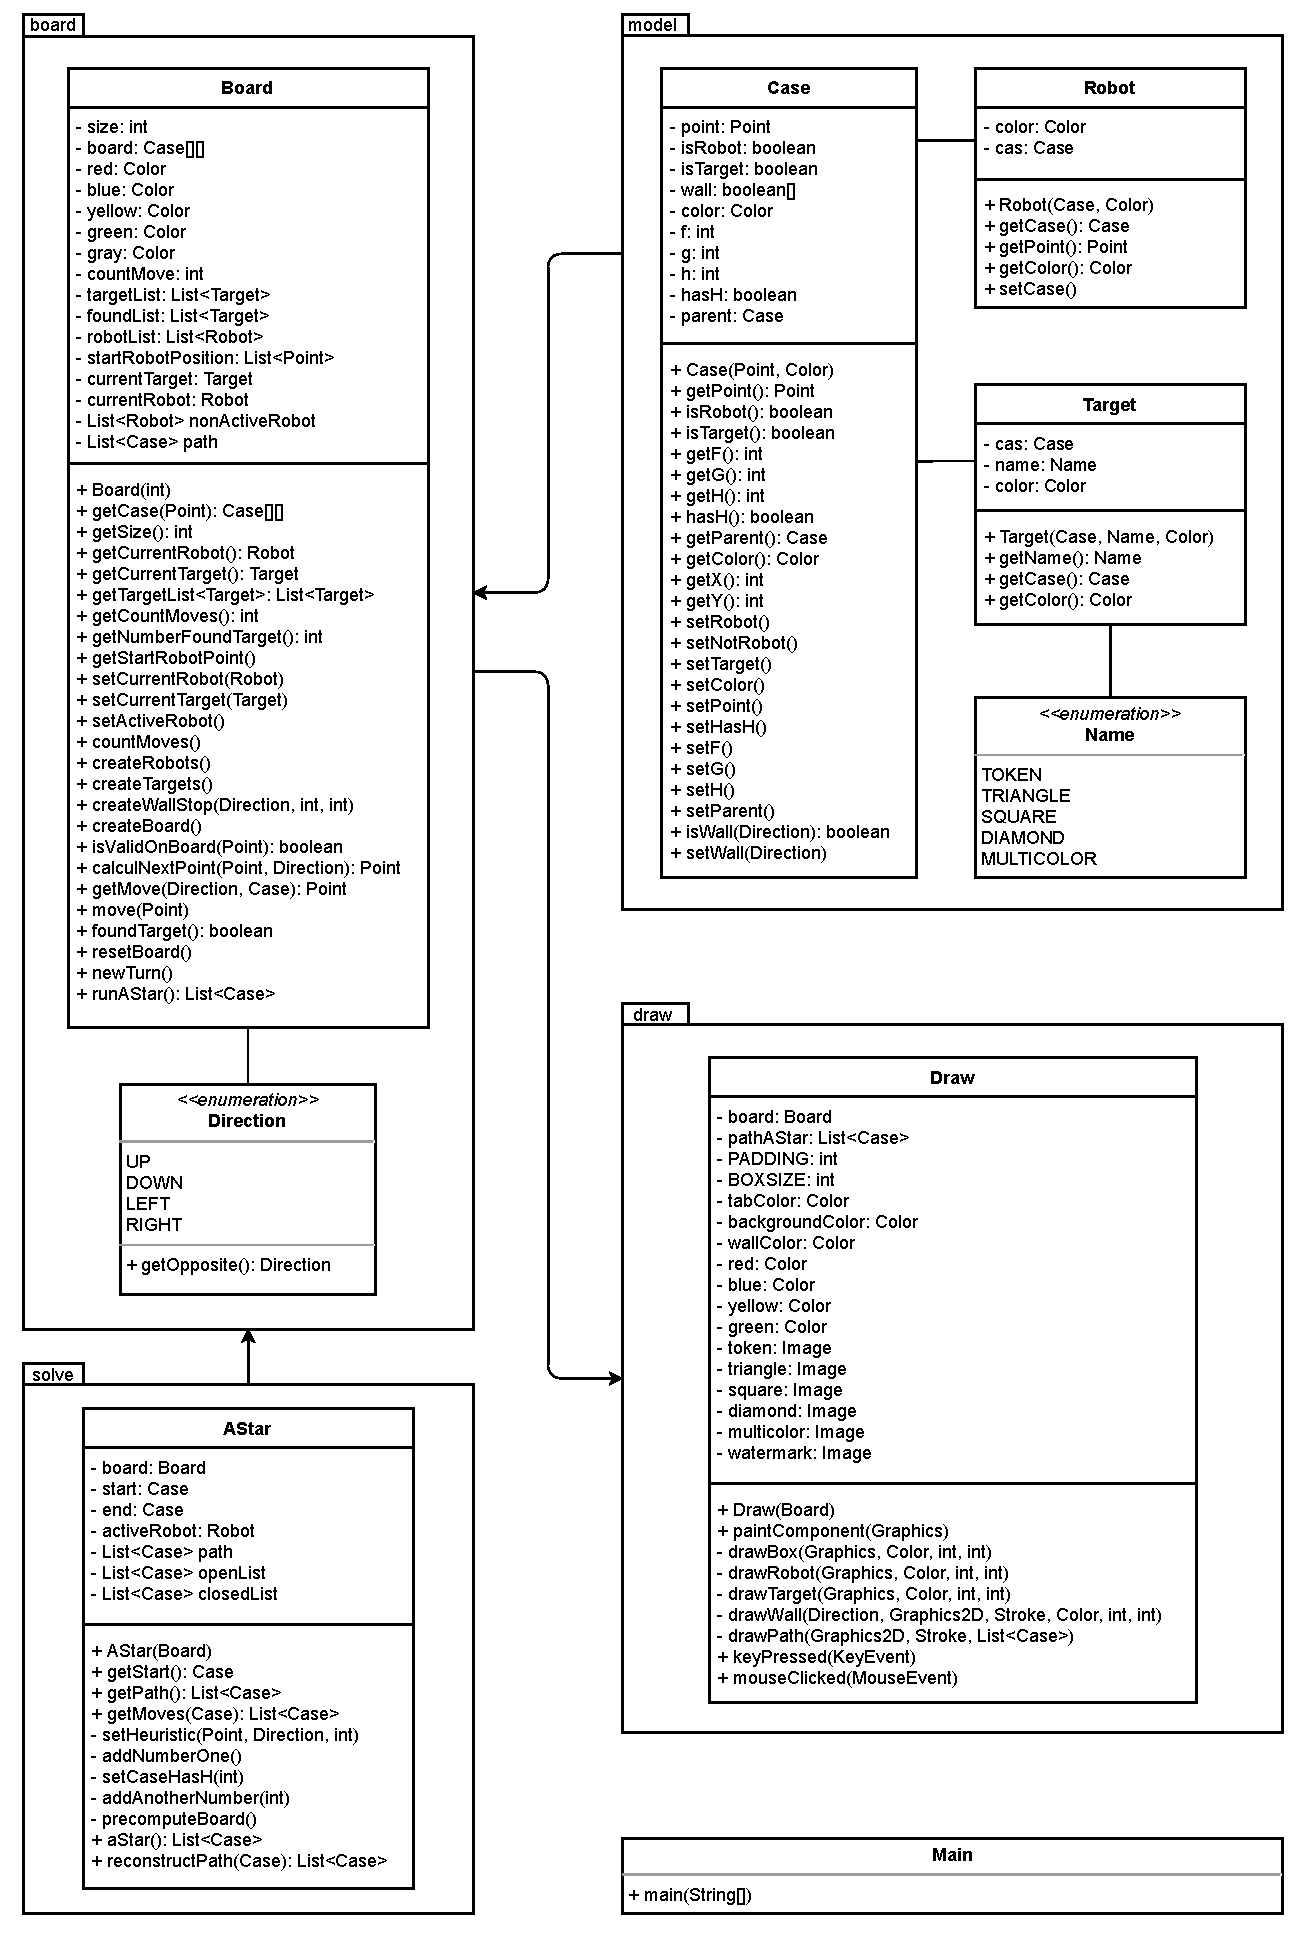
\includegraphics[width=0.95\textwidth]{sources/uml.pdf}
        \caption{Diagramme des classes}
    \end{figure}

\pagebreak

\section{Développement du projet}

    \subsection{Création du plateau}
    Au début, on sait que la taille du plateau est de 16x16, 256 carrées, 5 robots et 16 tuiles. Donc, on crée la classe des cases nommées \textbf{Case} qui sera une petite carrée du plateau. On trouve que le plateau a neuf cases différentes et les cases contiennent les tuiles ou les robots ou sont nulles. (Image à 4.3.2 - Figure 5)
    
    En effet, on utilise le booléen dans les cases pour contrôler les robots, les tuiles et les positions du mur. On a un commun des cases du mur, la possibilité d'avoir un mur en haut, en bas, à gauche et à droite avec le format de direction \texttt{\{up, down, left, right\}}. Par exemple, le mur en haut à la liste \texttt{\{true, false, false, false\}}, la case de robot est \texttt{true}, et la case de tuile est \texttt{true}. 
    
    \begin{figure}[H]
        \centering
        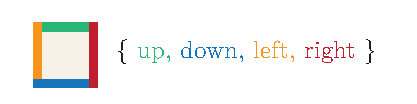
\includegraphics[width=0.7\textwidth]{sources/case-wall-ex.pdf}
        \caption{Format de direction}
    \end{figure}


    \begin{figure}[H]
        \centering
        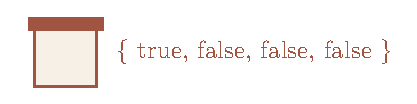
\includegraphics[width=0.7\textwidth]{sources/case-wall-ex2.pdf}
        \caption{Exemple d'une case}
    \end{figure}
    
    On initialise les robots dans la classe \textbf{Robot} avec les couleurs et les rôles qui se mettent en lien avec la classe \textbf{Case} par la méthode \texttt{setRobot():Case}. Avec les tuiles, on écrit une classe \textbf{Target} représentant les tuiles comme le robot, ajoute le nom de type et met en lien avec les cases en méthode \texttt{setTarget():Case}.
    
    Finalement, on construit le plateau avec les cases en défaut. Après avoir créé les cases sur le plateau, c'est à ce moment-là que l'on place les éléments qui sont les murs, les robots et les tuiles. On utilise une variable intermédiaire pour déterminer les robots et les tuiles dans la case après avoir créé et mettre dans un \texttt{ArrayList} de chaque type \texttt{Robot} ou \texttt{Target} pour les manager.
    

    \subsection{Déplacement et collision des robots}
    Selon aux règles du jeu, on déplace un robot vers une direction, ce robot se déplace jusqu’à ce qu'il rencontre un obstacle (le mur ou les autres robots). Grâce aux rôles des cases, on met la capacité de distinguer les obstacles dans ce robot pour le stopper. On construit le mur d'arrêt qui a deux directions opposées afin de contrôle la direction du robot.

    \begin{figure}[H]
        \centering
        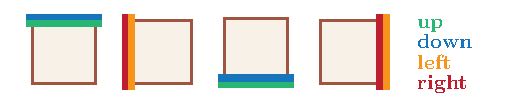
\includegraphics[width=0.7\textwidth]{sources/wall-stop.pdf}
        \caption{Cases avec murs pour stopper le robot}
    \end{figure}

    On contrôle la situation d'une case qui contient seulement un robot. C'est pourquoi le robot ne peut pas être dans une même case.


    \subsection{Design Pattern Modèle-Vue-Contrôleur (MVC)}
    Dans cette partie, on construit l'interface du jeu par la librairie Java Swing qui a été inclus au JDK depuis la version 1.2, cette libraire est moins compliquée d'installer que la librairie JavaFX, avec la conception Modèle-Vue-Contrôleur (MVC). Et on souhaite de ne pas lancer la ligne de commande quand on joue le jeu. 
    
    Java Swing\cite{swing} fait partie de la bibliothèque Java Foundation Classes (JFC). C'est un API dont le but est similaire à celui de l'API AWT, mais son fonctionnement et son utilisation sont complètement différentes.

    Modèle-Vue-Contrôleur ou MVC\cite{mvc} qui est composé de trois types de modules ayant trois responsabilités différentes : les modèles, les vues et les contrôleurs (un motif d'architecture logicielle destiné aux interfaces graphiques).

        \subsubsection{Modèle}
        Un modèle est les données à afficher. Par conséquent, on développe quatre classes de modèle qui sont \textbf{Case}, \textbf{Name}, \textbf{Robot} et \textbf{Target}.

        \subsubsection{Vue}
        Une vue présente l'interface graphique. Pour simplifier, on divise les murs à quatre cases de switch avec les directions et dessine en fonction \texttt{drawLine} et \texttt{setStroke} de la classe \textbf{Graphics2D}.

        \begin{figure}[H]
            \centering
            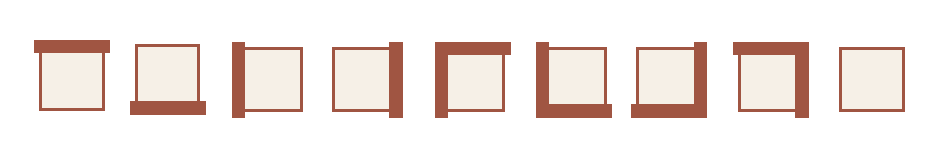
\includegraphics[width=1\textwidth]{sources/cases.pdf}
            \caption{Neuf cases avec mur}
        \end{figure}

        En outre, les robots sont des cercles et les targets sont des carrées avec les symboles différents. On va dessiner avec les fonctions principales \texttt{fillOval}, \texttt{fillRect} et \texttt{drawImage} de la classe \textbf{Graphics}

        \begin{figure}[H]
            \centering
            
\includegraphics[width=0.4\textwidth]{sources/graphic-1.pdf}
            \caption{Modèle d'un robot et d'une tuile de couleur bleu}
        \end{figure}

        C'est un jeu pour tout le monde, par suite on choisit le minimalisme avec
        une palette ci-dessous, car ce sont des couleurs douces et non sombres. Elles donnent une atmosphère relax quand on joue.
        \begin{figure}[H]
            \centering
            
\includegraphics[width=1\textwidth]{sources/palette.pdf}
            \caption{Palette de couleurs}
        \end{figure}

        En résumé, on indique les remarques de l'interface graphique sur l'image ci-dessous et "Mochi Shiba Pun Pun" qui apporte l'amusement et la chance devient l'icônes du jeu.
        \begin{figure}[H]
            \centering
            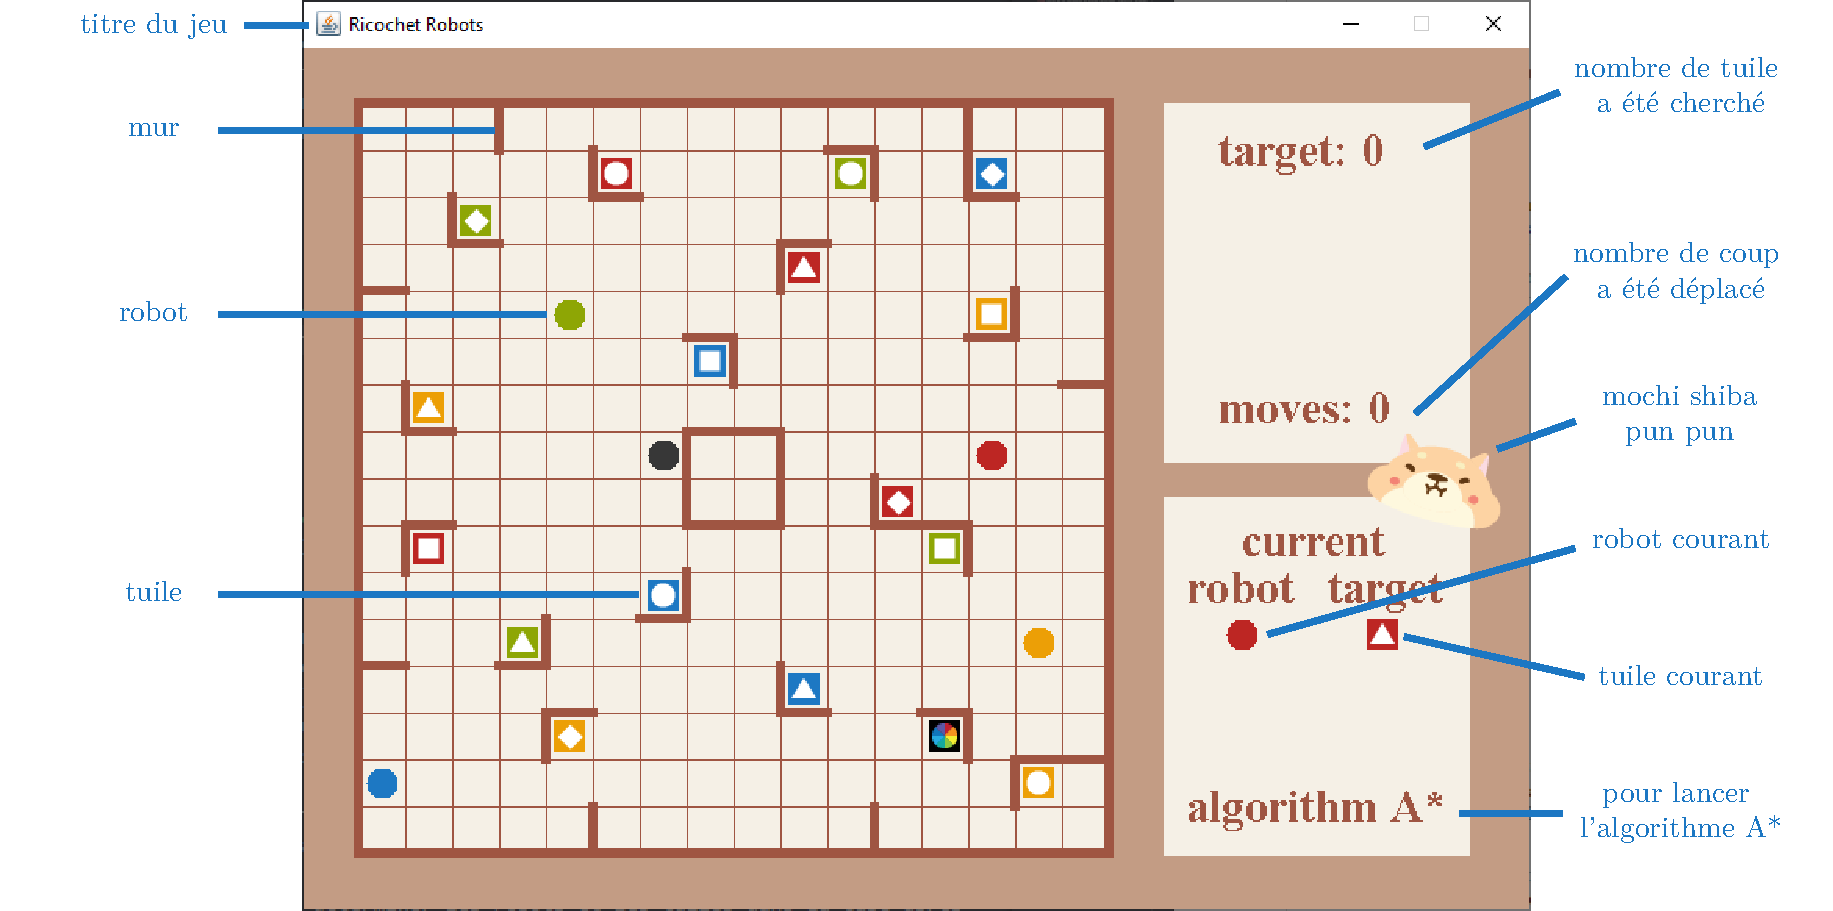
\includegraphics[width=1\textwidth]{sources/note.pdf}
            \caption{Remarques de l'interface graphique}
        \end{figure}

        \begin{figure}[H]
            \centering
            
\includegraphics[width=0.4\textwidth]{sources/chomap.pdf}
            \caption{"Mochi Shiba Pun Pun"}
        \end{figure}

        \subsubsection{Contrôleur}
        Un contrôleur contient la logique concernant les actions effectuées par l'utilisateur. Pour faire les contrôleurs, on doit implémenter des interfaces \textbf{ActionListener} et \textbf{KeyListener}.

        Premièrement, pour choisir les autres robots sur le plateau, on doit calculer le point de case par rapport les coordonnées de souris. Par exemple la coordonnée qui correspond au point de robot (4, 4) est de (170, 170). On propose la formule pour calculer le point (x, y) de robot de la coordonnée (xPos, yPos):
        \begin{align*}
            x = (xPos - PADDING) / BOXSIZE \\ 
            y = (yPos - PADDING) / BOXSIZE
        \end{align*}

        Deuxièmement, on met les conditions des coordonnées pouvant fonctionner dans les zones autorisées de la souris et utilise la méthode \texttt{mouseClicked(MouseEvent)} pour appeler la fonction de changement le robot et la fonction de recherche le chemin.

        Enfin, pour terminer cette partie, on met les méthodes de déplacer le robot, de compter les coupes et faire nouveau état du plateau quand les tuiles ont été cherchées dans les navigateurs de clavier avec la méthode \texttt{keyPressed(KeyEvent)}.
        



\pagebreak

\section{Algorithme A*}
Intelligence artificielle peut résoudre des problèmes d'une énorme complexité combinatoire. Dans Ricochet Robots, un robot doit chercher la tuile cible de même couleur que l'on l'a tiré. De plus, pour aider les joueurs qui peuvent trouver facilement la solution du jeu, on construit une fonction avec l'algorithme A*. Cet algorithme doit être très simple, ne nécessite pas de prétraitement et consomme très peu de mémoire.
    
    \subsection{Présentation d'algorithme A*}
    Algorithme A*\cite{wikialgo} est un algorithme de recherche de chemin dans un graphe pondéré : à partir d'un nœud de départ spécifique d'un graphique, il vise à trouver un chemin vers le nœud de but donné ayant le plus petit coût (distance-la moins parcourue, temps le plus court, etc). A* est basé sur l'utilisation de méthodes heuristiques pour atteindre l'optimalisé et l'exhaustivité et est une variante de l'algorithme best-first.

    Il faut conserver un arbre de chemins provenant du nœud de départ et en étendant ces chemins un bord à la fois jusqu'à ce que son critère de terminaison soit satisfait. À chaque itération de sa boucle principale, A* doit déterminer le chemin à développer. Il le fait en fonction du coût du chemin et d'une estimation du coût requis pour étendre le chemin vers la cible. Plus précisément, l'algorithme choisit le plus petit chemin.

    Lorsqu'un algorithme de recherche a la propriété d'optimalisé, cela signifie qu'il est garanti de trouver la meilleure solution possible, dans notre cas le chemin le plus court vers l'état d'arriver. Et quand un algorithme de recherche a la propriété d'exhaustivité, cela signifie que s'il existe une solution à un problème donné, l'algorithme est assuré de la trouver. 
    
    \subsection{Algorithme de parcours en largeur}

        On utilise les cases \texttt{c} de classe \textbf{Case} qui contient les valeurs des fonctions $f(c)$, $g(c)$ et $h(c)$ comme un noeud de l'algorithme. 
        
        \subsubsection{Fonction de coût \texorpdfstring{$f(c)$}{f(c)}}
        On veut déterminer dans quelle case se déplacer à chaque étape. Pour ce faire, on va concevoir une fonction mathématique $f(c)$ qui mesurera à quel point une case candidate est bonne pour être inclus dans notre chemin le plus court.

        C'est la fonction de coût et on veut la minimiser pour produire un résultat optimal. La fonction de coût est la somme d'une fonction de déplacement et d'une fonction heuristique.
        \begin{align*}
            f(c) = g(c) + h(c)
        \end{align*}

        \subsubsection{Fonction de déplacement \texorpdfstring{$g(c)$}{g(c)}}
        On appelle cette fonction de déplacement $g(c)$ est de 0 en défaut. $g(c)$ est la distance parcourue entre la case de départ A et la case courante. Ainsi, les cases voisins de la case de départ auront une distance qui est la longueur entre le case de départ et eux.

        Pour calculer $g(c)$, on obtient les coordonnées $g(c)$ de la case avant la case actuelle, la distance entre la case précédente et la case actuelle. Chaque case a sa propre valeur $g(c)$ de la case de départ à cette case.

        \subsubsection{Fonction heuristique \texorpdfstring{$h(c)$}{h(c)}}
        La fonction heuristique est utilisée pour estimer à quel point la case que l'on examine est proche de la cible. On choisit l'heuristique grâce au diaporama de Michael Fogleman \cite{heuristic} et à la présentation de Randy Coulman \cite{youtube}. 

        D'abord, on a une liste d'états à prendre en compte au lieu de choisir simplement celui qui a la plus courte distance. On ajoute un facteur qui est une estimation de combien on reste à parcourir et tant que cette estimation n'est jamais une surestimation. On peut en quelque sorte calculer si les robots pourraient s'arrêter n'importe où où ils le voulaient, combien de mouvements ont pris pour atteindre la tuile si évidemment.

        Sur le plateau, l'heuristique des cases $h(c)$ en défaut est de 0, on commence à partir du robot au choix et doit déjà aller c'est 0 tout en ligne droite est un 1 tout en ligne droite à partir de là il y a un 2 puis 3, 4 et 5 et dans ce plateau $h(c)$ est de jusqu’à 5.

        \begin{figure}[H]
            \centering
            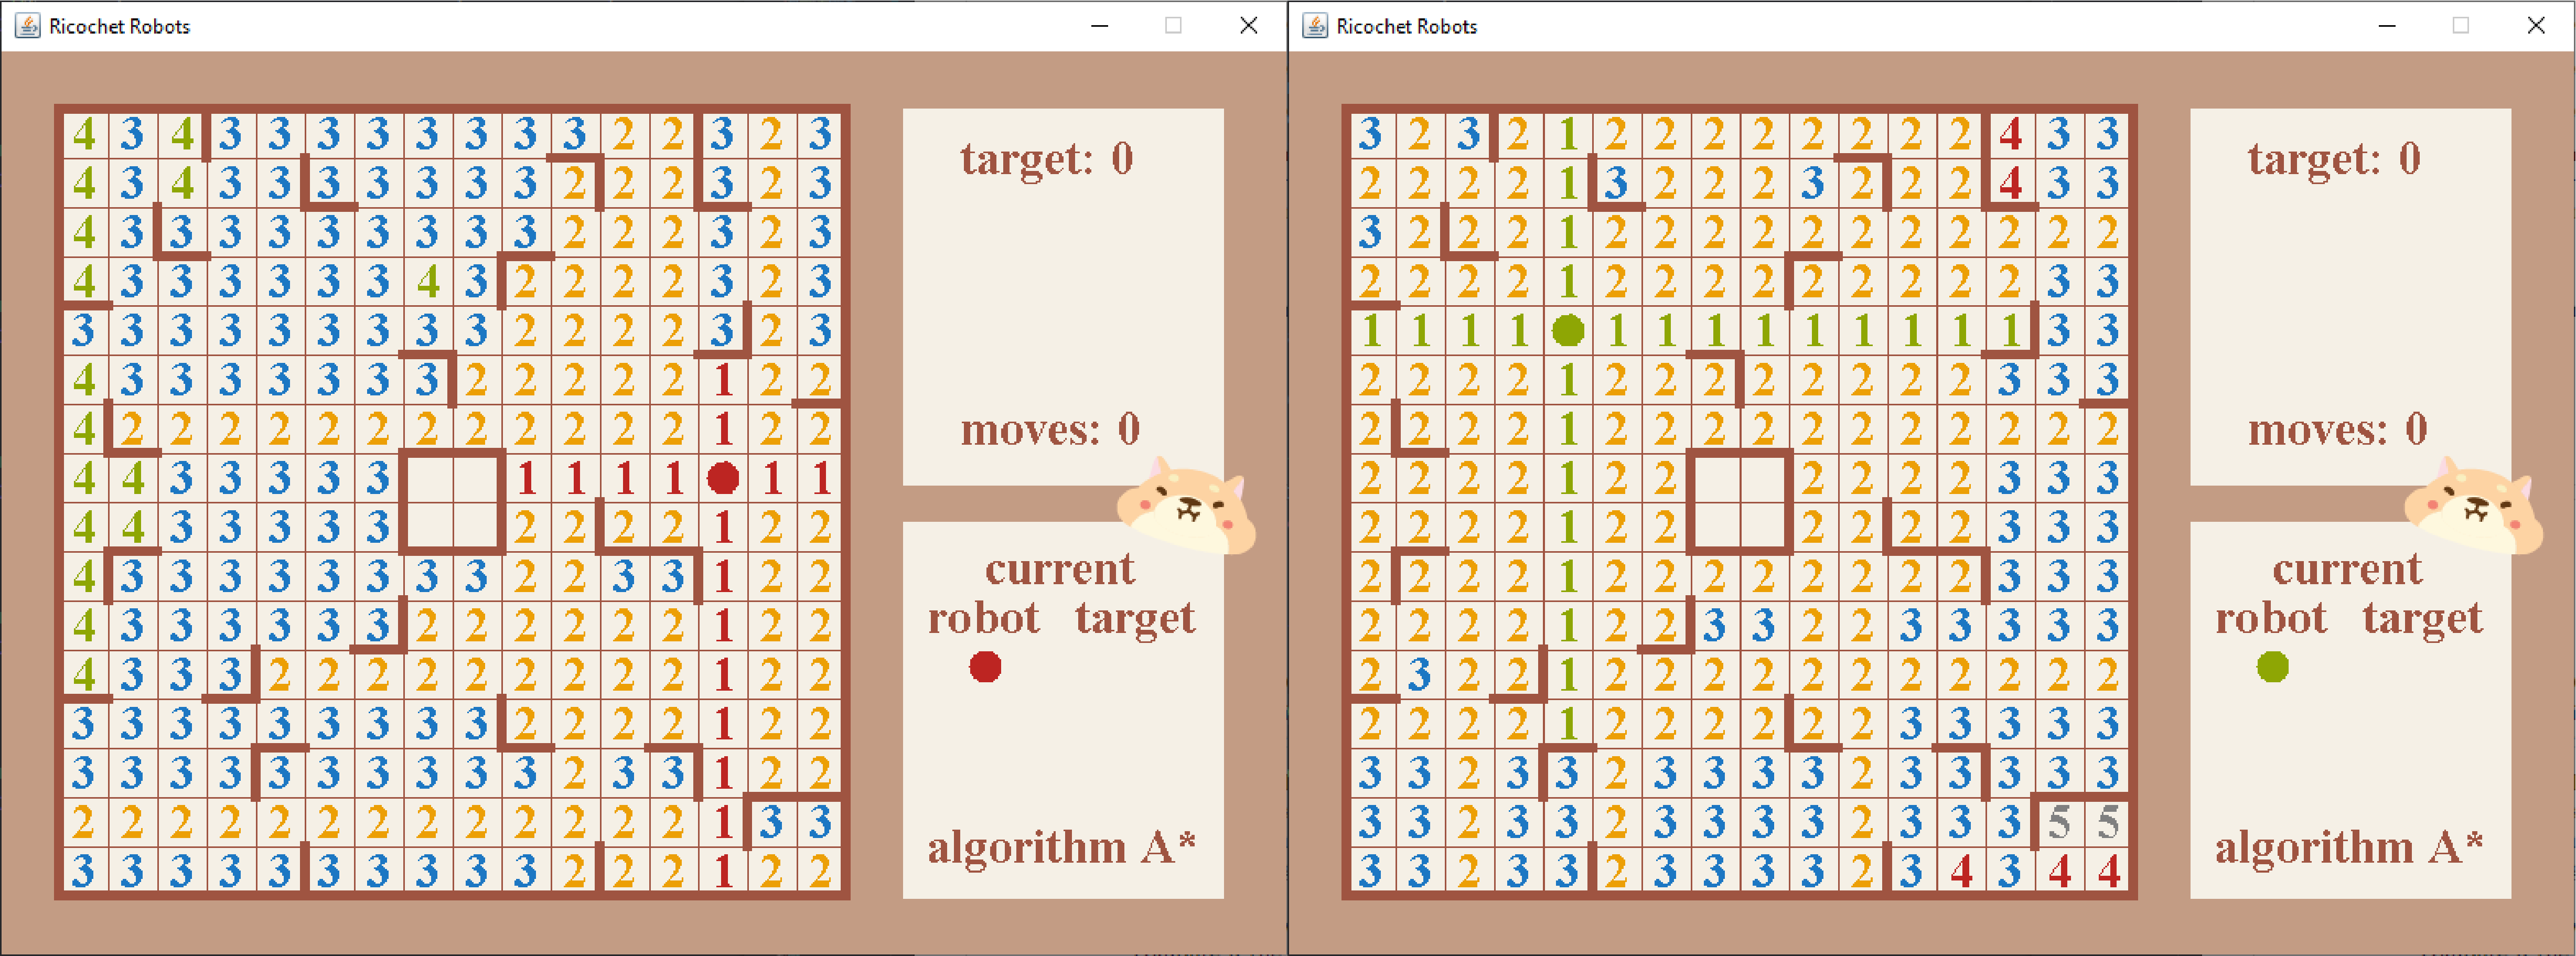
\includegraphics[width=1\textwidth]{sources/heuristic.png}
            \caption{Affichage des valeurs heuristiques}
        \end{figure}

        Donc, à partir de ces cases marquées cinq, même si les robots pouvaient s'arrêter où ils le souhaitent, il faudrait cinq mouvements pour entrer dans la case de but à partir de là, à cause de la structure du plateau et de l'emplacement des murs.

    \subsection{Implémentation d'algorithme A*}
    Premièrement, on crée la méthode \texttt{aStar(): List<Case>} pour construit l'algorithme. On simplifie la zone de recherche pour gestion plus facile. On divise la zone de recherche en cases. Chaque case est un élément de l'algorithme.

    Deuxièmement, on doit avoir 2 list :
    \begin{itemize}
        \item Un pour l'enregistrement de tous les cases que l'on doit examiner pour trouver le chemin le plus court (\texttt{openList}).
        \item Un pour l'enregistrement de tous les cases que l'on n'a pas besoin de revoir (\texttt{closedList}).
    \end{itemize} 
    
    Troisièmement, on ajoute la position de la case de départ à \texttt{closedList}. Aussi, ajouter tous les cases que le robot peut arriver de la position actuelle à \texttt{openList}. N'oubliez pas que ce n'est pas un obstacle.

    Maintenant, on calcule la valeur du chemin et met une valeur de $f(c)$ à chaque case. Ici, on examine seulement que la case ne peut aller qu'en droit entre la case.

    Pour trouver le chemin le plus court, on répète les étapes suivantes: 
    \begin{itemize}
        \item Prendre la case en \texttt{openList} avec une valeur $f(c)$ minimale. Appeler cela la case B.
        \item Supprimer B de \texttt{openList} et ajouter B à \texttt{closedList}.
        \item Si M est la liste des cases que B peut déplacer (des coups validés), alors soit I est l'examen de chaque case dans M.
        \item Si I est déjà dans \texttt{closedList}, ignorer.
        \item Si I n'est pas dans \texttt{openList}, ajouter-le pour calculer les valeurs de distance.
        \item Si I est dans \texttt{openList}: vérifier-le, si la valeur $f(c)$ est moins à la valeur $f(c)$ du point actuel, de même mettre à jour le nouveau point actuel.
    \end{itemize}

    Pour conclure, on écrit une méthode \texttt{reconstructPath(Case):List<Case>} pour obtenir la chemin final par rapport aux cases parents lorsque la case courant a le même point à la case de la tuile courant.




\pagebreak

\section{Instruction du jeu}
    \subsection{Lancer le jeu}
    Il y a beaucoup du logiciel de construction automatisée d’application qui automatisent la création d'applications exécutables à partir du code source sur la marché comme ANT, Maven et Gradle. Sur ce projet, on décide d'utiliser le Gradle, car c'est simple pour écrire le script et pour lancer.

    Entrez la commande \texttt{./gradlew run} pour lancer le jeu. Ça fonctionne avec le Linux Shell et Windows Powershell.

    \subsection{Jouer le jeu}
    
    \begin{figure}[H]
        \centering
        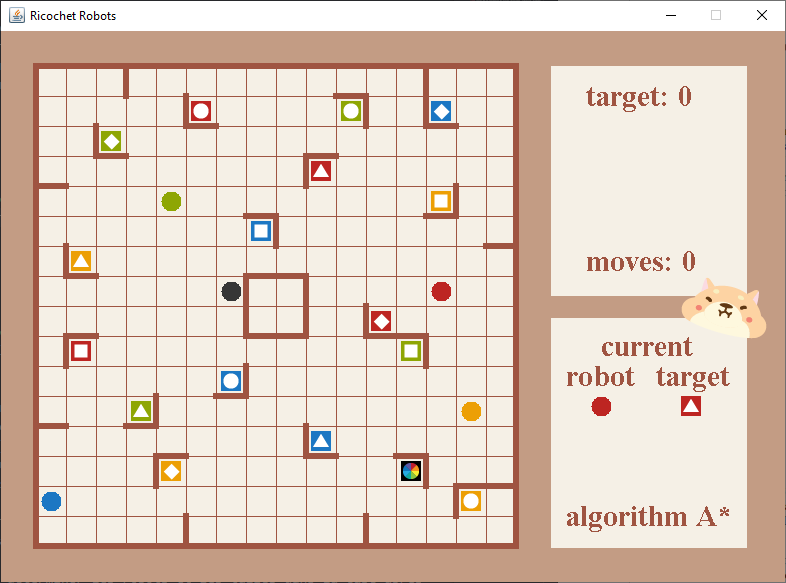
\includegraphics[width=0.7\textwidth]{sources/cap-1.png}
        \caption{Initialisation du plateau}
    \end{figure}

    On utilise quatre navigateurs sur le clavier pour déplacer les robots. On note si le clavier ne fonctionne pas, relancer le jeu. Ensuite, pour changer le robot courant, on clique sur les autres robots. Pour l'algorithme A*, cliquez sur le texte "algorithme A*" sur écran, les chemins vont afficher et le robot peut déplacer sur ces chemins.





\pagebreak

\section{Captures d'écran}
\begin{figure}[H]
    \centering
    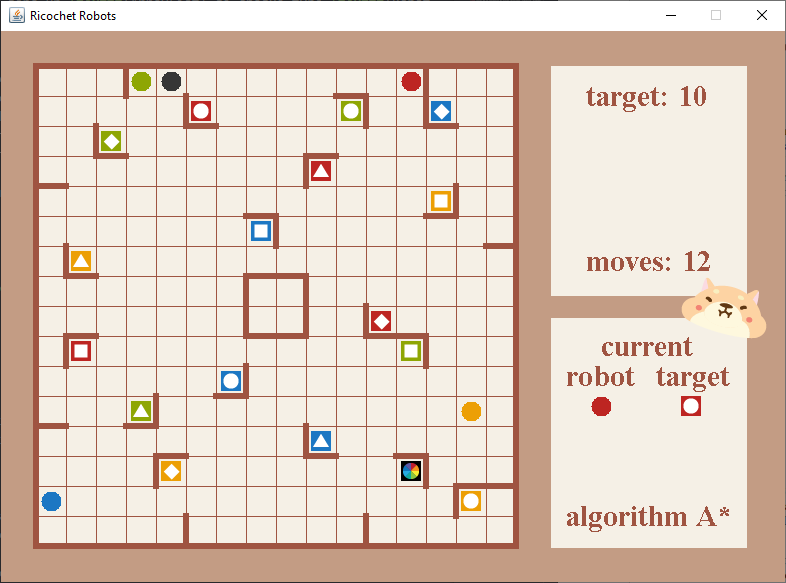
\includegraphics[width=0.7\textwidth]{sources/cap-2.png}
    \caption{Jouer en normal}
\end{figure}

\begin{figure}[H]
    \centering
    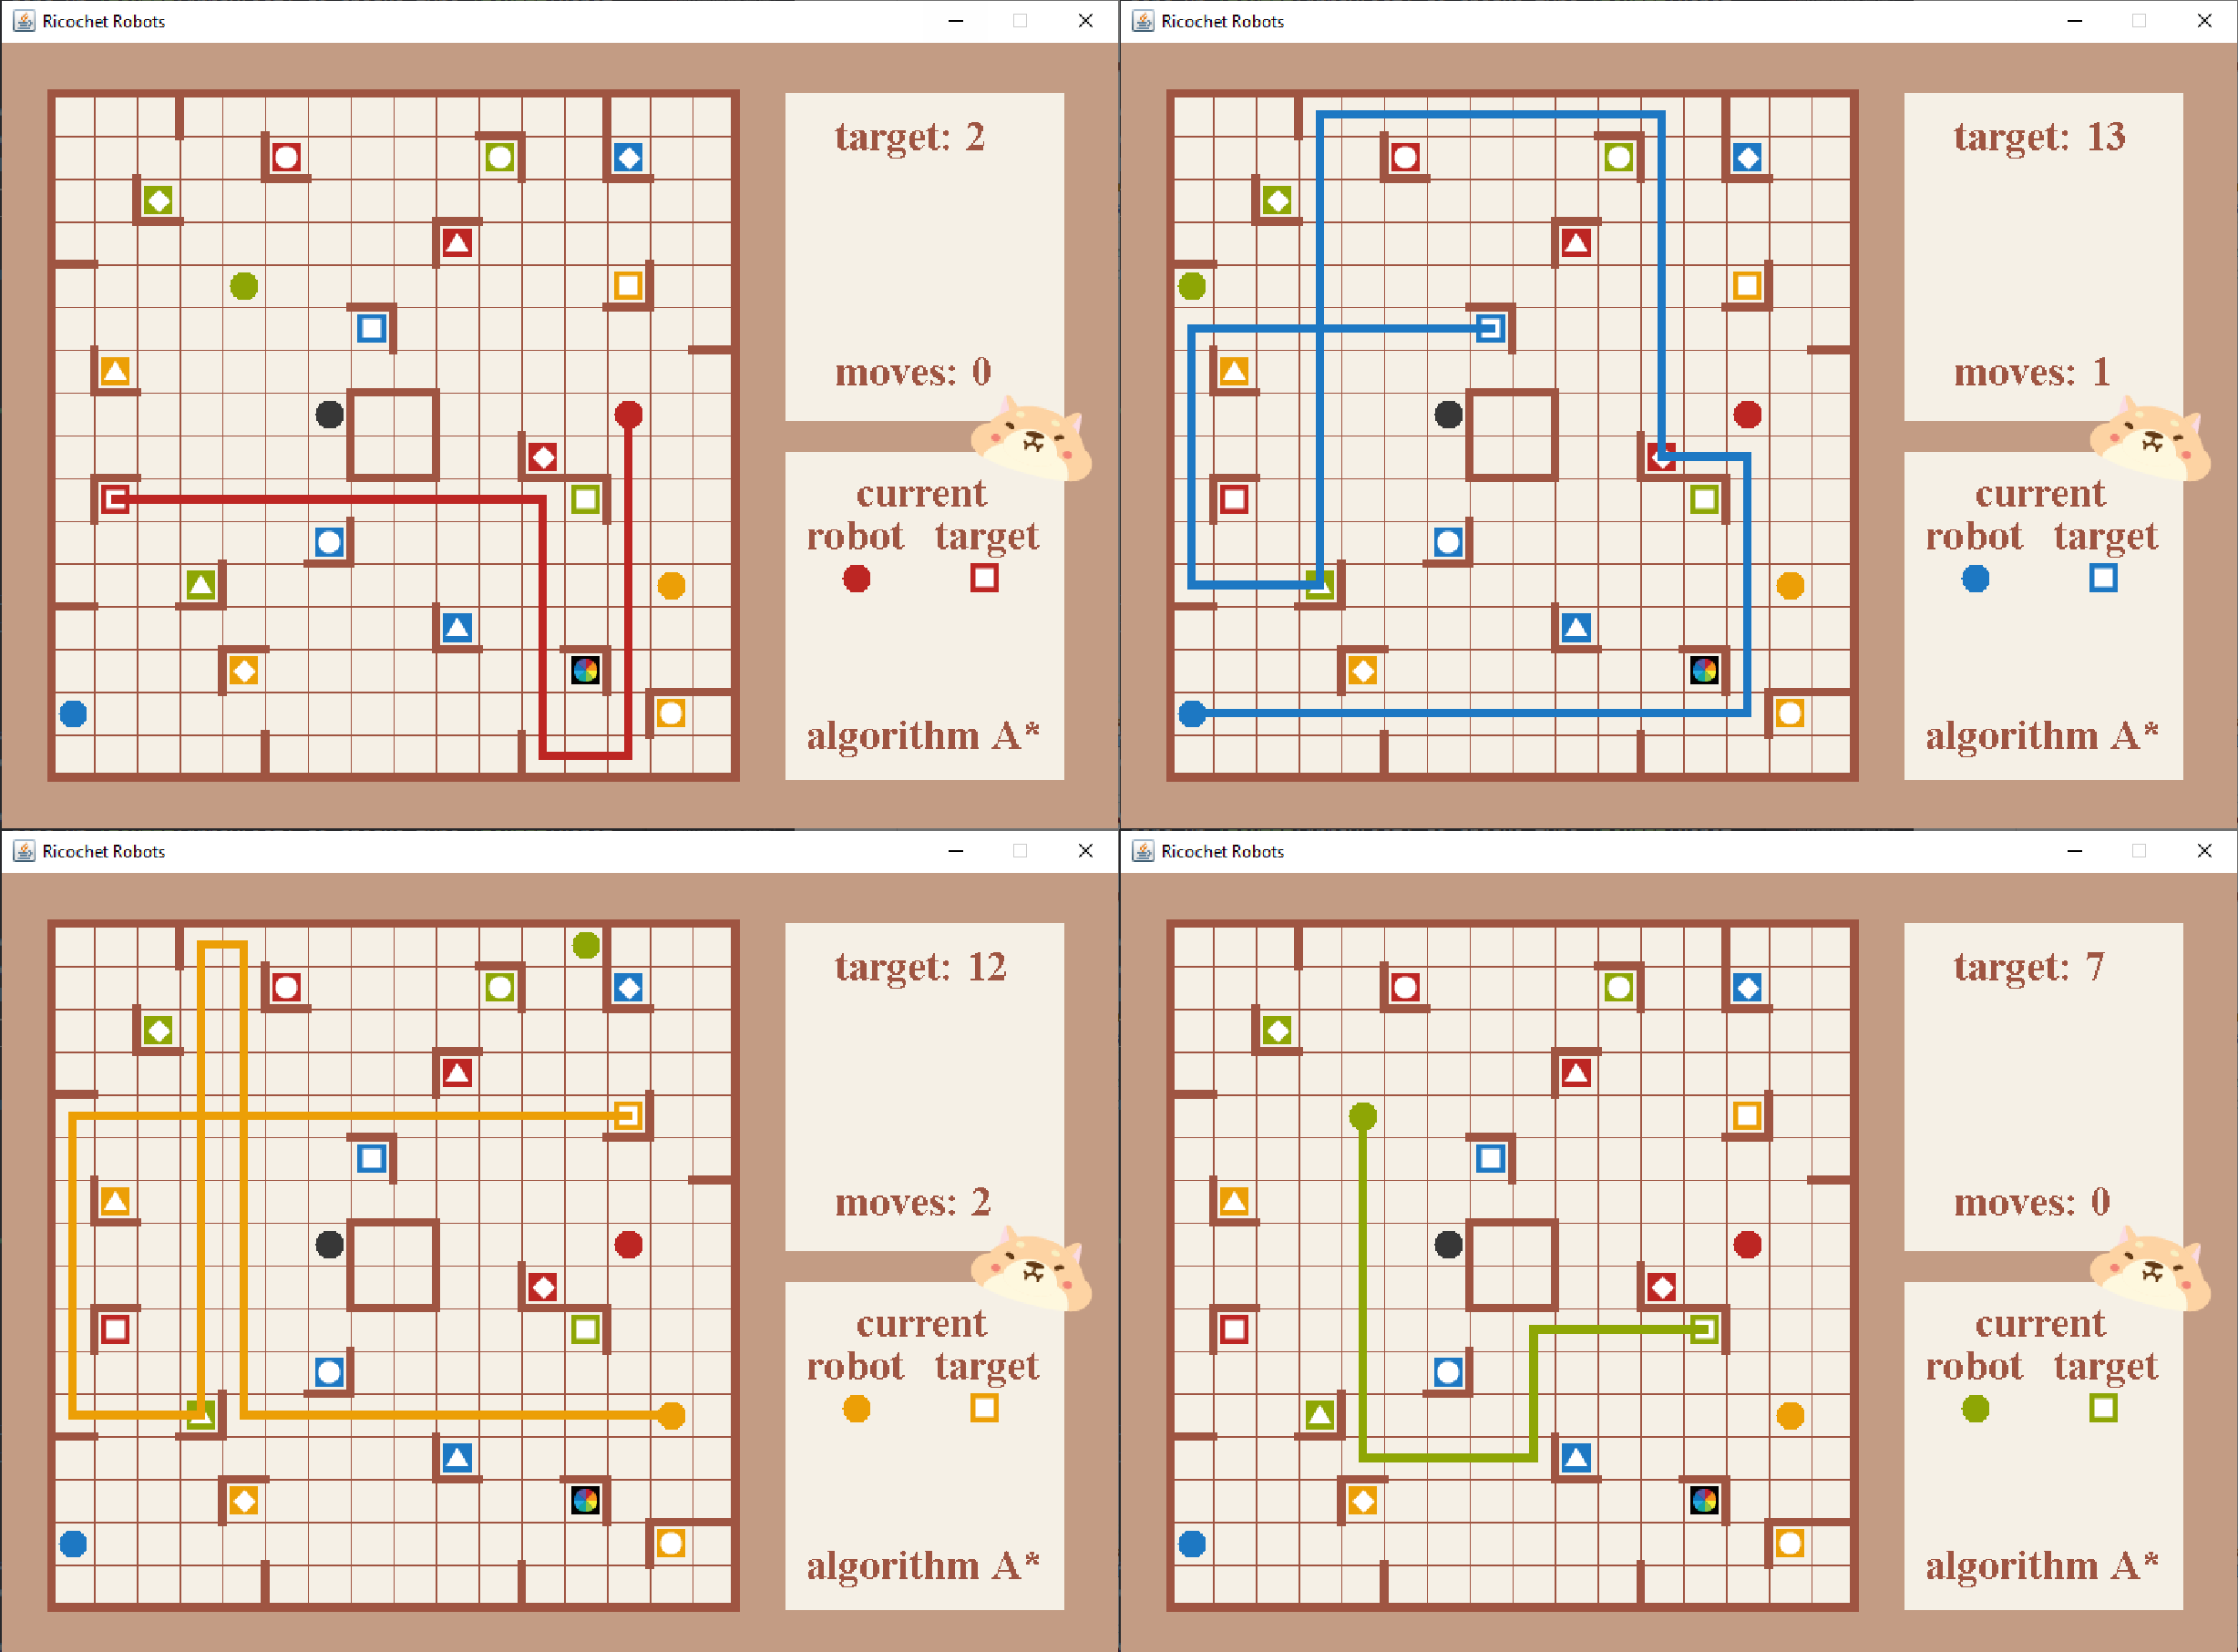
\includegraphics[width=1\textwidth]{sources/cap-algo.pdf}
    \caption{Jouer avec algorithme A*}
\end{figure}

\pagebreak

\section{Conclusion}
Après ce projet, j'ai mieux compris la libraire Java Swing, le Java Build Tools Gradle, comment l'algorithme A* fonctionne et le jeu de société Ricochet Robots, je n'ai pas connu ce jeu en précédent. En autre, j'ai avancé la capacité de débugger, d'optimiser le code avec la conception MVC. Malgré que je n'aie pas fini la partie de déplacer multi-robots avec l'algorithme A*, je continuerai de terminer.

Enfin, je veux remercier Mme DHAOU de me conseiller pendant les cours de travaux pratiques ainsi que M. BONNET pour ses cours magistraux. Merci d'avoir pris le temps de lire ce rapport.

\pagebreak

\bibliographystyle{unsrt}
\bibliography{bibliography}

\end{document}